\documentclass[1p]{elsarticle_modified}
%\bibliographystyle{elsarticle-num}

%\usepackage[colorlinks]{hyperref}
%\usepackage{abbrmath_seonhwa} %\Abb, \Ascr, \Acal ,\Abf, \Afrak
\usepackage{amsfonts}
\usepackage{amssymb}
\usepackage{amsmath}
\usepackage{amsthm}
\usepackage{scalefnt}
\usepackage{amsbsy}
\usepackage{kotex}
\usepackage{caption}
\usepackage{subfig}
\usepackage{color}
\usepackage{graphicx}
\usepackage{xcolor} %% white, black, red, green, blue, cyan, magenta, yellow
\usepackage{float}
\usepackage{setspace}
\usepackage{hyperref}

\usepackage{tikz}
\usetikzlibrary{arrows}

\usepackage{multirow}
\usepackage{array} % fixed length table
\usepackage{hhline}

%%%%%%%%%%%%%%%%%%%%%
\makeatletter
\renewcommand*\env@matrix[1][\arraystretch]{%
	\edef\arraystretch{#1}%
	\hskip -\arraycolsep
	\let\@ifnextchar\new@ifnextchar
	\array{*\c@MaxMatrixCols c}}
\makeatother %https://tex.stackexchange.com/questions/14071/how-can-i-increase-the-line-spacing-in-a-matrix
%%%%%%%%%%%%%%%

\usepackage[normalem]{ulem}

\newcommand{\msout}[1]{\ifmmode\text{\sout{\ensuremath{#1}}}\else\sout{#1}\fi}
%SOURCE: \msout is \stkout macro in https://tex.stackexchange.com/questions/20609/strikeout-in-math-mode

\newcommand{\cancel}[1]{
	\ifmmode
	{\color{red}\msout{#1}}
	\else
	{\color{red}\sout{#1}}
	\fi
}

\newcommand{\add}[1]{
	{\color{blue}\uwave{#1}}
}

\newcommand{\replace}[2]{
	\ifmmode
	{\color{red}\msout{#1}}{\color{blue}\uwave{#2}}
	\else
	{\color{red}\sout{#1}}{\color{blue}\uwave{#2}}
	\fi
}

\newcommand{\Sol}{\mathcal{S}} %segment
\newcommand{\D}{D} %diagram
\newcommand{\A}{\mathcal{A}} %arc


%%%%%%%%%%%%%%%%%%%%%%%%%%%%%5 test

\def\sl{\operatorname{\textup{SL}}(2,\Cbb)}
\def\psl{\operatorname{\textup{PSL}}(2,\Cbb)}
\def\quan{\mkern 1mu \triangleright \mkern 1mu}

\theoremstyle{definition}
\newtheorem{thm}{Theorem}[section]
\newtheorem{prop}[thm]{Proposition}
\newtheorem{lem}[thm]{Lemma}
\newtheorem{ques}[thm]{Question}
\newtheorem{cor}[thm]{Corollary}
\newtheorem{defn}[thm]{Definition}
\newtheorem{exam}[thm]{Example}
\newtheorem{rmk}[thm]{Remark}
\newtheorem{alg}[thm]{Algorithm}

\newcommand{\I}{\sqrt{-1}}
\begin{document}

%\begin{frontmatter}
%
%\title{Boundary parabolic representations of knots up to 8 crossings}
%
%%% Group authors per affiliation:
%\author{Yunhi Cho} 
%\address{Department of Mathematics, University of Seoul, Seoul, Korea}
%\ead{yhcho@uos.ac.kr}
%
%
%\author{Seonhwa Kim} %\fnref{s_kim}}
%\address{Center for Geometry and Physics, Institute for Basic Science, Pohang, 37673, Korea}
%\ead{ryeona17@ibs.re.kr}
%
%\author{Hyuk Kim}
%\address{Department of Mathematical Sciences, Seoul National University, Seoul 08826, Korea}
%\ead{hyukkim@snu.ac.kr}
%
%\author{Seokbeom Yoon}
%\address{Department of Mathematical Sciences, Seoul National University, Seoul, 08826,  Korea}
%\ead{sbyoon15@snu.ac.kr}
%
%\begin{abstract}
%We find all boundary parabolic representation of knots up to 8 crossings.
%
%\end{abstract}
%\begin{keyword}
%    \MSC[2010] 57M25 
%\end{keyword}
%
%\end{frontmatter}

%\linenumbers
%\tableofcontents
%
\newcommand\colored[1]{\textcolor{white}{\rule[-0.35ex]{0.8em}{1.4ex}}\kern-0.8em\color{red} #1}%
%\newcommand\colored[1]{\textcolor{white}{ #1}\kern-2.17ex	\textcolor{white}{ #1}\kern-1.81ex	\textcolor{white}{ #1}\kern-2.15ex\color{red}#1	}

{\Large $\underline{11a_{137}~(K11a_{137})}$}

\setlength{\tabcolsep}{10pt}
\renewcommand{\arraystretch}{1.6}
\vspace{1cm}\begin{tabular}{m{100pt}>{\centering\arraybackslash}m{274pt}}
\multirow{5}{120pt}{
	\centering
	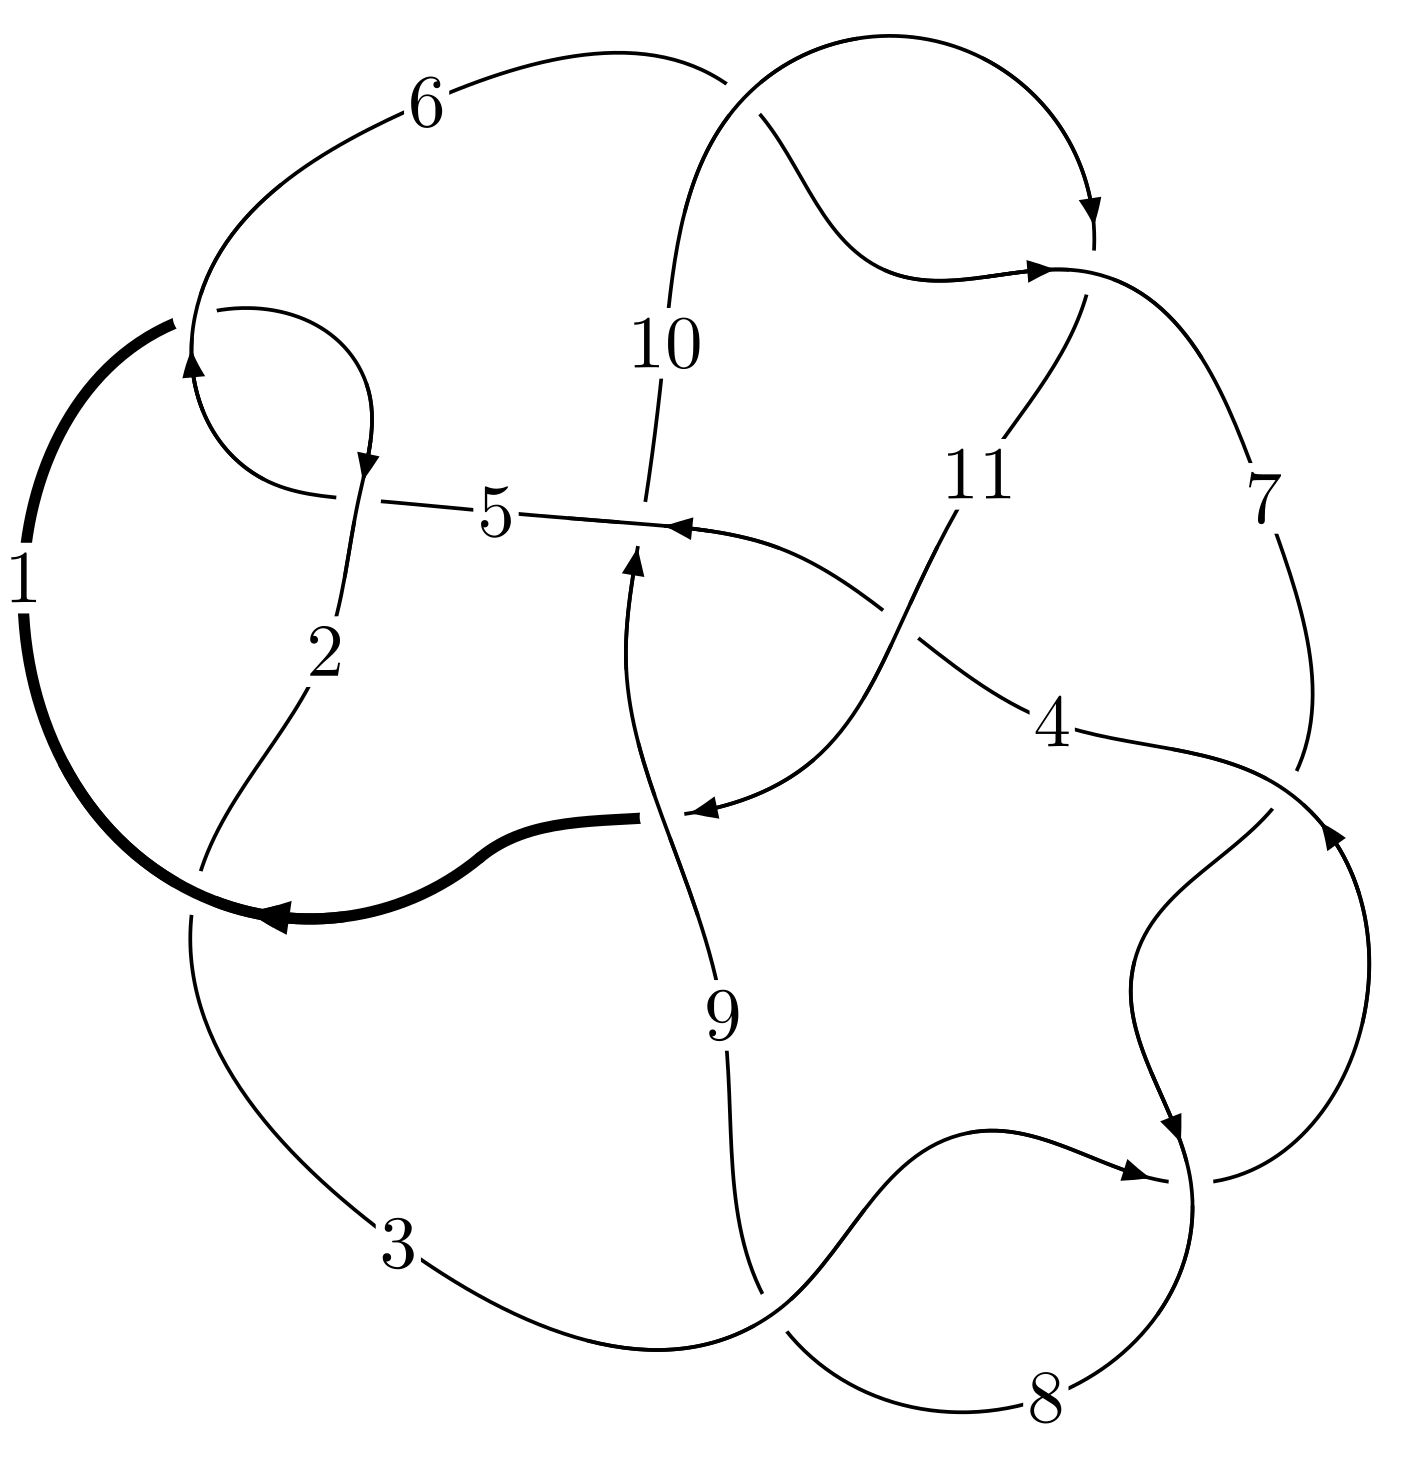
\includegraphics[width=112pt]{../../../GIT/diagram.site/Diagrams/png/386_11a_137.png}\\
\ \ \ A knot diagram\footnotemark}&
\allowdisplaybreaks
\textbf{Linearized knot diagam} \\
\cline{2-2}
 &
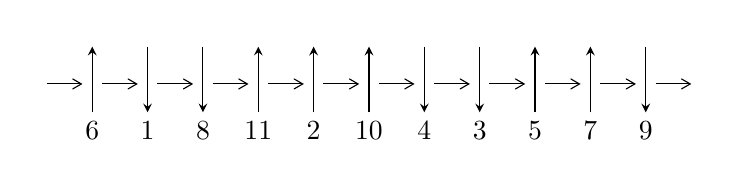
\begin{tikzpicture}[x=20pt, y=17pt]
	% nodes
	\node (C0) at (0, 0) {};
	\node (C1) at (1, 0) {};
	\node (C1U) at (1, +1) {};
	\node (C1D) at (1, -1) {6};

	\node (C2) at (2, 0) {};
	\node (C2U) at (2, +1) {};
	\node (C2D) at (2, -1) {1};

	\node (C3) at (3, 0) {};
	\node (C3U) at (3, +1) {};
	\node (C3D) at (3, -1) {8};

	\node (C4) at (4, 0) {};
	\node (C4U) at (4, +1) {};
	\node (C4D) at (4, -1) {11};

	\node (C5) at (5, 0) {};
	\node (C5U) at (5, +1) {};
	\node (C5D) at (5, -1) {2};

	\node (C6) at (6, 0) {};
	\node (C6U) at (6, +1) {};
	\node (C6D) at (6, -1) {10};

	\node (C7) at (7, 0) {};
	\node (C7U) at (7, +1) {};
	\node (C7D) at (7, -1) {4};

	\node (C8) at (8, 0) {};
	\node (C8U) at (8, +1) {};
	\node (C8D) at (8, -1) {3};

	\node (C9) at (9, 0) {};
	\node (C9U) at (9, +1) {};
	\node (C9D) at (9, -1) {5};

	\node (C10) at (10, 0) {};
	\node (C10U) at (10, +1) {};
	\node (C10D) at (10, -1) {7};

	\node (C11) at (11, 0) {};
	\node (C11U) at (11, +1) {};
	\node (C11D) at (11, -1) {9};
	\node (C12) at (12, 0) {};

	% arrows
	\draw[->,>={angle 60}]
	(C0) edge (C1) (C1) edge (C2) (C2) edge (C3) (C3) edge (C4) (C4) edge (C5) (C5) edge (C6) (C6) edge (C7) (C7) edge (C8) (C8) edge (C9) (C9) edge (C10) (C10) edge (C11) (C11) edge (C12) ;	\draw[->,>=stealth]
	(C1D) edge (C1U) (C2U) edge (C2D) (C3U) edge (C3D) (C4D) edge (C4U) (C5D) edge (C5U) (C6D) edge (C6U) (C7U) edge (C7D) (C8U) edge (C8D) (C9D) edge (C9U) (C10D) edge (C10U) (C11U) edge (C11D) ;
	\end{tikzpicture} \\
\hhline{~~} \\& 
\textbf{Solving Sequence} \\ \cline{2-2} 
 &
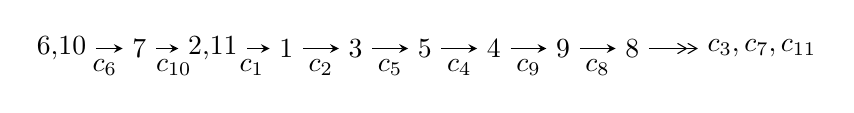
\begin{tikzpicture}[x=25pt, y=7pt]
	% node
	\node (A0) at (-1/8, 0) {6,10};
	\node (A1) at (1, 0) {7};
	\node (A2) at (33/16, 0) {2,11};
	\node (A3) at (25/8, 0) {1};
	\node (A4) at (33/8, 0) {3};
	\node (A5) at (41/8, 0) {5};
	\node (A6) at (49/8, 0) {4};
	\node (A7) at (57/8, 0) {9};
	\node (A8) at (65/8, 0) {8};
	\node (C1) at (1/2, -1) {$c_{6}$};
	\node (C2) at (3/2, -1) {$c_{10}$};
	\node (C3) at (21/8, -1) {$c_{1}$};
	\node (C4) at (29/8, -1) {$c_{2}$};
	\node (C5) at (37/8, -1) {$c_{5}$};
	\node (C6) at (45/8, -1) {$c_{4}$};
	\node (C7) at (53/8, -1) {$c_{9}$};
	\node (C8) at (61/8, -1) {$c_{8}$};
	\node (A9) at (10, 0) {$c_{3},c_{7},c_{11}$};

	% edge
	\draw[->,>=stealth]	
	(A0) edge (A1) (A1) edge (A2) (A2) edge (A3) (A3) edge (A4) (A4) edge (A5) (A5) edge (A6) (A6) edge (A7) (A7) edge (A8) ;
	\draw[->>,>={angle 60}]	
	(A8) edge (A9);
\end{tikzpicture} \\ 

\end{tabular} \\

\footnotetext{
The image of knot diagram is generated by the software ``\textbf{Draw programme}" developed by Andrew Bartholomew(\url{http://www.layer8.co.uk/maths/draw/index.htm\#Running-draw}), where we modified some parts for our purpose(\url{https://github.com/CATsTAILs/LinksPainter}).
}\phantom \\ \newline 
\centering \textbf{Ideals for irreducible components\footnotemark of $X_{\text{par}}$} 
 
\begin{align*}
I^u_{1}&=\langle 
2.62286\times10^{122} u^{66}-5.83233\times10^{122} u^{65}+\cdots+8.34384\times10^{121} b+3.23422\times10^{123},\\
\phantom{I^u_{1}}&\phantom{= \langle  }7.89658\times10^{122} u^{66}-1.90489\times10^{123} u^{65}+\cdots+5.84069\times10^{122} a+4.77578\times10^{123},\\
\phantom{I^u_{1}}&\phantom{= \langle  }u^{67}- u^{66}+\cdots+178 u+14\rangle \\
I^u_{2}&=\langle 
u^6- u^5-3 u^4+3 u^3+3 u^2+b-2 u-1,\\
\phantom{I^u_{2}}&\phantom{= \langle  }- u^{11}+2 u^{10}+5 u^9-12 u^8-9 u^7+31 u^6+4 u^5-43 u^4+8 u^3+31 u^2+2 a-10 u-9,\\
\phantom{I^u_{2}}&\phantom{= \langle  }u^{12}-2 u^{11}-5 u^{10}+12 u^9+9 u^8-29 u^7-6 u^6+35 u^5-21 u^3+5 u+2\rangle \\
\\
\end{align*}
\raggedright * 2 irreducible components of $\dim_{\mathbb{C}}=0$, with total 79 representations.\\
\footnotetext{All coefficients of polynomials are rational numbers. But the coefficients are sometimes approximated in decimal forms when there is not enough margin.}
\newpage
\renewcommand{\arraystretch}{1}
\centering \section*{I. $I^u_{1}= \langle 2.62\times10^{122} u^{66}-5.83\times10^{122} u^{65}+\cdots+8.34\times10^{121} b+3.23\times10^{123},\;7.90\times10^{122} u^{66}-1.90\times10^{123} u^{65}+\cdots+5.84\times10^{122} a+4.78\times10^{123},\;u^{67}- u^{66}+\cdots+178 u+14 \rangle$}
\flushleft \textbf{(i) Arc colorings}\\
\begin{tabular}{m{7pt} m{180pt} m{7pt} m{180pt} }
\flushright $a_{6}=$&$\begin{pmatrix}1\\0\end{pmatrix}$ \\
\flushright $a_{10}=$&$\begin{pmatrix}0\\u\end{pmatrix}$ \\
\flushright $a_{7}=$&$\begin{pmatrix}1\\- u^2\end{pmatrix}$ \\
\flushright $a_{2}=$&$\begin{pmatrix}-1.35200 u^{66}+3.26141 u^{65}+\cdots-118.518 u-8.17674\\-3.14346 u^{66}+6.98998 u^{65}+\cdots-456.720 u-38.7618\end{pmatrix}$ \\
\flushright $a_{11}=$&$\begin{pmatrix}u\\- u^3+u\end{pmatrix}$ \\
\flushright $a_{1}=$&$\begin{pmatrix}1.79147 u^{66}-3.72857 u^{65}+\cdots+338.203 u+30.5851\\-3.14346 u^{66}+6.98998 u^{65}+\cdots-456.720 u-38.7618\end{pmatrix}$ \\
\flushright $a_{3}=$&$\begin{pmatrix}6.35511 u^{66}-14.1634 u^{65}+\cdots+956.320 u+88.5224\\-5.13936 u^{66}+11.5473 u^{65}+\cdots-761.528 u-66.6848\end{pmatrix}$ \\
\flushright $a_{5}=$&$\begin{pmatrix}1.65994 u^{66}-3.47429 u^{65}+\cdots+303.006 u+31.5407\\-5.11342 u^{66}+11.2674 u^{65}+\cdots-724.107 u-63.0777\end{pmatrix}$ \\
\flushright $a_{4}=$&$\begin{pmatrix}8.11928 u^{66}-17.8617 u^{65}+\cdots+1164.71 u+104.265\\-8.57661 u^{66}+18.9928 u^{65}+\cdots-1183.18 u-101.347\end{pmatrix}$ \\
\flushright $a_{9}=$&$\begin{pmatrix}-1.57345 u^{66}+3.70563 u^{65}+\cdots-91.7422 u-2.61257\\2.16777 u^{66}-4.87111 u^{65}+\cdots+235.385 u+18.0302\end{pmatrix}$ \\
\flushright $a_{8}=$&$\begin{pmatrix}4.14278 u^{66}-9.73696 u^{65}+\cdots+392.893 u+31.7183\\-6.68802 u^{66}+15.1248 u^{65}+\cdots-868.092 u-73.9457\end{pmatrix}$\\ \flushright $a_{8}=$&$\begin{pmatrix}4.14278 u^{66}-9.73696 u^{65}+\cdots+392.893 u+31.7183\\-6.68802 u^{66}+15.1248 u^{65}+\cdots-868.092 u-73.9457\end{pmatrix}$\\&\end{tabular}
\flushleft \textbf{(ii) Obstruction class $= -1$}\\~\\
\flushleft \textbf{(iii) Cusp Shapes $= 15.0826 u^{66}-33.1683 u^{65}+\cdots+1975.74 u+173.234$}\\~\\
\newpage\renewcommand{\arraystretch}{1}
\flushleft \textbf{(iv) u-Polynomials at the component}\newline \\
\begin{tabular}{m{50pt}|m{274pt}}
Crossings & \hspace{64pt}u-Polynomials at each crossing \\
\hline $$\begin{aligned}c_{1},c_{5}\end{aligned}$$&$\begin{aligned}
&u^{67}+12 u^{65}+\cdots+23 u+1
\end{aligned}$\\
\hline $$\begin{aligned}c_{2}\end{aligned}$$&$\begin{aligned}
&u^{67}+24 u^{66}+\cdots+655 u-1
\end{aligned}$\\
\hline $$\begin{aligned}c_{3},c_{7},c_{8}\end{aligned}$$&$\begin{aligned}
&u^{67}+u^{66}+\cdots+34 u-11
\end{aligned}$\\
\hline $$\begin{aligned}c_{4}\end{aligned}$$&$\begin{aligned}
&u^{67}-3 u^{66}+\cdots-56360 u+14843
\end{aligned}$\\
\hline $$\begin{aligned}c_{6},c_{10}\end{aligned}$$&$\begin{aligned}
&u^{67}+u^{66}+\cdots+178 u-14
\end{aligned}$\\
\hline $$\begin{aligned}c_{9}\end{aligned}$$&$\begin{aligned}
&u^{67}+u^{66}+\cdots+1218 u-523
\end{aligned}$\\
\hline $$\begin{aligned}c_{11}\end{aligned}$$&$\begin{aligned}
&u^{67}-11 u^{66}+\cdots+19734 u-3697
\end{aligned}$\\
\hline
\end{tabular}\\~\\
\newpage\renewcommand{\arraystretch}{1}
\flushleft \textbf{(v) Riley Polynomials at the component}\newline \\
\begin{tabular}{m{50pt}|m{274pt}}
Crossings & \hspace{64pt}Riley Polynomials at each crossing \\
\hline $$\begin{aligned}c_{1},c_{5}\end{aligned}$$&$\begin{aligned}
&y^{67}+24 y^{66}+\cdots+655 y-1
\end{aligned}$\\
\hline $$\begin{aligned}c_{2}\end{aligned}$$&$\begin{aligned}
&y^{67}+44 y^{66}+\cdots+467315 y-1
\end{aligned}$\\
\hline $$\begin{aligned}c_{3},c_{7},c_{8}\end{aligned}$$&$\begin{aligned}
&y^{67}+73 y^{66}+\cdots-5026 y-121
\end{aligned}$\\
\hline $$\begin{aligned}c_{4}\end{aligned}$$&$\begin{aligned}
&y^{67}-31 y^{66}+\cdots+4845129346 y-220314649
\end{aligned}$\\
\hline $$\begin{aligned}c_{6},c_{10}\end{aligned}$$&$\begin{aligned}
&y^{67}-59 y^{66}+\cdots+2144 y-196
\end{aligned}$\\
\hline $$\begin{aligned}c_{9}\end{aligned}$$&$\begin{aligned}
&y^{67}-19 y^{66}+\cdots+1068262 y-273529
\end{aligned}$\\
\hline $$\begin{aligned}c_{11}\end{aligned}$$&$\begin{aligned}
&y^{67}+25 y^{66}+\cdots-401527606 y-13667809
\end{aligned}$\\
\hline
\end{tabular}\\~\\
\newpage\flushleft \textbf{(vi) Complex Volumes and Cusp Shapes}
$$\begin{array}{c|c|c}  
\text{Solutions to }I^u_{1}& \I (\text{vol} + \sqrt{-1}CS) & \text{Cusp shape}\\
 \hline 
\begin{aligned}
u &= -0.142657 + 0.992860 I \\
a &= \phantom{-}0.56636 + 1.48377 I \\
b &= \phantom{-}0.033263 + 1.144420 I\end{aligned}
 & \phantom{-}1.70877 + 2.32867 I & \phantom{-0.000000 } 0 \\ \hline\begin{aligned}
u &= -0.142657 - 0.992860 I \\
a &= \phantom{-}0.56636 - 1.48377 I \\
b &= \phantom{-}0.033263 - 1.144420 I\end{aligned}
 & \phantom{-}1.70877 - 2.32867 I & \phantom{-0.000000 } 0 \\ \hline\begin{aligned}
u &= -0.099779 + 1.006020 I \\
a &= -0.20395 - 1.63071 I \\
b &= \phantom{-}0.623398 - 0.982401 I\end{aligned}
 & -0.20027 - 6.31062 I & \phantom{-0.000000 } 0 \\ \hline\begin{aligned}
u &= -0.099779 - 1.006020 I \\
a &= -0.20395 + 1.63071 I \\
b &= \phantom{-}0.623398 + 0.982401 I\end{aligned}
 & -0.20027 + 6.31062 I & \phantom{-0.000000 } 0 \\ \hline\begin{aligned}
u &= -0.981096 + 0.054455 I \\
a &= -0.76387 - 1.69840 I \\
b &= -0.044418 - 0.942425 I\end{aligned}
 & \phantom{-}0.0186179 + 0.0387429 I & \phantom{-0.000000 } 0 \\ \hline\begin{aligned}
u &= -0.981096 - 0.054455 I \\
a &= -0.76387 + 1.69840 I \\
b &= -0.044418 + 0.942425 I\end{aligned}
 & \phantom{-}0.0186179 - 0.0387429 I & \phantom{-0.000000 } 0 \\ \hline\begin{aligned}
u &= -0.270773 + 0.833923 I \\
a &= \phantom{-}0.195059 + 0.748297 I \\
b &= \phantom{-}0.604424 + 0.639267 I\end{aligned}
 & \phantom{-}0.80579 - 1.40750 I & \phantom{-0.000000 -}0. + 4.43919 I \\ \hline\begin{aligned}
u &= -0.270773 - 0.833923 I \\
a &= \phantom{-}0.195059 - 0.748297 I \\
b &= \phantom{-}0.604424 - 0.639267 I\end{aligned}
 & \phantom{-}0.80579 + 1.40750 I & \phantom{-0.000000 } 0. - 4.43919 I \\ \hline\begin{aligned}
u &= \phantom{-}1.107010 + 0.303823 I \\
a &= \phantom{-}0.50610 - 1.37239 I \\
b &= -0.121641 - 1.174720 I\end{aligned}
 & -0.89603 + 4.38119 I & \phantom{-0.000000 } 0 \\ \hline\begin{aligned}
u &= \phantom{-}1.107010 - 0.303823 I \\
a &= \phantom{-}0.50610 + 1.37239 I \\
b &= -0.121641 + 1.174720 I\end{aligned}
 & -0.89603 - 4.38119 I & \phantom{-0.000000 } 0\\
 \hline 
 \end{array}$$\newpage$$\begin{array}{c|c|c}  
\text{Solutions to }I^u_{1}& \I (\text{vol} + \sqrt{-1}CS) & \text{Cusp shape}\\
 \hline 
\begin{aligned}
u &= \phantom{-}1.136800 + 0.224242 I \\
a &= \phantom{-}0.966929 - 0.878075 I \\
b &= -0.740988 - 1.111300 I\end{aligned}
 & \phantom{-}2.93656 + 4.60816 I & \phantom{-0.000000 } 0 \\ \hline\begin{aligned}
u &= \phantom{-}1.136800 - 0.224242 I \\
a &= \phantom{-}0.966929 + 0.878075 I \\
b &= -0.740988 + 1.111300 I\end{aligned}
 & \phantom{-}2.93656 - 4.60816 I & \phantom{-0.000000 } 0 \\ \hline\begin{aligned}
u &= \phantom{-}1.224370 + 0.009584 I \\
a &= \phantom{-}0.293275 + 0.010079 I \\
b &= -0.933790 + 0.466037 I\end{aligned}
 & \phantom{-}4.82838 - 1.51282 I & \phantom{-0.000000 } 0 \\ \hline\begin{aligned}
u &= \phantom{-}1.224370 - 0.009584 I \\
a &= \phantom{-}0.293275 - 0.010079 I \\
b &= -0.933790 - 0.466037 I\end{aligned}
 & \phantom{-}4.82838 + 1.51282 I & \phantom{-0.000000 } 0 \\ \hline\begin{aligned}
u &= \phantom{-}1.104740 + 0.538484 I \\
a &= \phantom{-}0.98881 + 1.60795 I \\
b &= -0.048348 + 0.578810 I\end{aligned}
 & \phantom{-}7.98310 + 2.39539 I & \phantom{-0.000000 } 0 \\ \hline\begin{aligned}
u &= \phantom{-}1.104740 - 0.538484 I \\
a &= \phantom{-}0.98881 - 1.60795 I \\
b &= -0.048348 - 0.578810 I\end{aligned}
 & \phantom{-}7.98310 - 2.39539 I & \phantom{-0.000000 } 0 \\ \hline\begin{aligned}
u &= -1.246690 + 0.004314 I \\
a &= -0.902444 - 0.638257 I \\
b &= \phantom{-}0.86616 - 1.20415 I\end{aligned}
 & \phantom{-}9.42380 - 4.94858 I & \phantom{-0.000000 } 0 \\ \hline\begin{aligned}
u &= -1.246690 - 0.004314 I \\
a &= -0.902444 + 0.638257 I \\
b &= \phantom{-}0.86616 + 1.20415 I\end{aligned}
 & \phantom{-}9.42380 + 4.94858 I & \phantom{-0.000000 } 0 \\ \hline\begin{aligned}
u &= \phantom{-}0.424436 + 1.177450 I \\
a &= \phantom{-}0.101432 + 0.607388 I \\
b &= -0.768711 + 0.568168 I\end{aligned}
 & \phantom{-}7.58682 + 3.59183 I & \phantom{-0.000000 } 0 \\ \hline\begin{aligned}
u &= \phantom{-}0.424436 - 1.177450 I \\
a &= \phantom{-}0.101432 - 0.607388 I \\
b &= -0.768711 - 0.568168 I\end{aligned}
 & \phantom{-}7.58682 - 3.59183 I & \phantom{-0.000000 } 0\\
 \hline 
 \end{array}$$\newpage$$\begin{array}{c|c|c}  
\text{Solutions to }I^u_{1}& \I (\text{vol} + \sqrt{-1}CS) & \text{Cusp shape}\\
 \hline 
\begin{aligned}
u &= -1.244190 + 0.216049 I \\
a &= \phantom{-}1.84039 + 1.27405 I \\
b &= -0.662475 + 0.965347 I\end{aligned}
 & \phantom{-}3.73550 - 4.99700 I & \phantom{-0.000000 } 0 \\ \hline\begin{aligned}
u &= -1.244190 - 0.216049 I \\
a &= \phantom{-}1.84039 - 1.27405 I \\
b &= -0.662475 - 0.965347 I\end{aligned}
 & \phantom{-}3.73550 + 4.99700 I & \phantom{-0.000000 } 0 \\ \hline\begin{aligned}
u &= -1.267400 + 0.140376 I \\
a &= -0.324635 + 0.014077 I \\
b &= \phantom{-}1.231450 - 0.468321 I\end{aligned}
 & \phantom{-}11.62150 - 2.40537 I & \phantom{-0.000000 } 0 \\ \hline\begin{aligned}
u &= -1.267400 - 0.140376 I \\
a &= -0.324635 - 0.014077 I \\
b &= \phantom{-}1.231450 + 0.468321 I\end{aligned}
 & \phantom{-}11.62150 + 2.40537 I & \phantom{-0.000000 } 0 \\ \hline\begin{aligned}
u &= \phantom{-}1.275090 + 0.042068 I \\
a &= -1.97186 - 0.47485 I \\
b &= \phantom{-}0.704366 - 0.840178 I\end{aligned}
 & \phantom{-}11.39430 + 0.35805 I & \phantom{-0.000000 } 0 \\ \hline\begin{aligned}
u &= \phantom{-}1.275090 - 0.042068 I \\
a &= -1.97186 + 0.47485 I \\
b &= \phantom{-}0.704366 + 0.840178 I\end{aligned}
 & \phantom{-}11.39430 - 0.35805 I & \phantom{-0.000000 } 0 \\ \hline\begin{aligned}
u &= \phantom{-}0.275788 + 0.662423 I \\
a &= -1.09829 + 1.97732 I \\
b &= \phantom{-}0.088329 + 0.994872 I\end{aligned}
 & -3.44236 - 0.72466 I & -6.99887 + 1.47430 I \\ \hline\begin{aligned}
u &= \phantom{-}0.275788 - 0.662423 I \\
a &= -1.09829 - 1.97732 I \\
b &= \phantom{-}0.088329 - 0.994872 I\end{aligned}
 & -3.44236 + 0.72466 I & -6.99887 - 1.47430 I \\ \hline\begin{aligned}
u &= -1.28332\phantom{ +0.000000I} \\
a &= -0.480905\phantom{ +0.000000I} \\
b &= \phantom{-}0.0382466\phantom{ +0.000000I}\end{aligned}
 & \phantom{-}2.83439\phantom{ +0.000000I} & \phantom{-0.000000 } 0 \\ \hline\begin{aligned}
u &= -1.290700 + 0.141599 I \\
a &= \phantom{-}0.109094 + 0.820721 I \\
b &= -0.682399 - 0.719924 I\end{aligned}
 & \phantom{-}4.48457 + 0.21946 I & \phantom{-0.000000 } 0\\
 \hline 
 \end{array}$$\newpage$$\begin{array}{c|c|c}  
\text{Solutions to }I^u_{1}& \I (\text{vol} + \sqrt{-1}CS) & \text{Cusp shape}\\
 \hline 
\begin{aligned}
u &= -1.290700 - 0.141599 I \\
a &= \phantom{-}0.109094 - 0.820721 I \\
b &= -0.682399 + 0.719924 I\end{aligned}
 & \phantom{-}4.48457 - 0.21946 I & \phantom{-0.000000 } 0 \\ \hline\begin{aligned}
u &= -1.223810 + 0.441106 I \\
a &= -0.440377 - 1.113580 I \\
b &= \phantom{-}0.263799 - 1.354580 I\end{aligned}
 & \phantom{-}5.11820 - 7.37502 I & \phantom{-0.000000 } 0 \\ \hline\begin{aligned}
u &= -1.223810 - 0.441106 I \\
a &= -0.440377 + 1.113580 I \\
b &= \phantom{-}0.263799 + 1.354580 I\end{aligned}
 & \phantom{-}5.11820 + 7.37502 I & \phantom{-0.000000 } 0 \\ \hline\begin{aligned}
u &= -0.642398 + 0.199393 I \\
a &= \phantom{-}2.73814 + 0.59347 I \\
b &= -0.329606 + 0.827830 I\end{aligned}
 & -1.07794 - 1.38861 I & \phantom{-}3.80624 + 5.85827 I \\ \hline\begin{aligned}
u &= -0.642398 - 0.199393 I \\
a &= \phantom{-}2.73814 - 0.59347 I \\
b &= -0.329606 - 0.827830 I\end{aligned}
 & -1.07794 + 1.38861 I & \phantom{-}3.80624 - 5.85827 I \\ \hline\begin{aligned}
u &= \phantom{-}1.372630 + 0.064390 I \\
a &= -0.790042 - 0.625685 I \\
b &= \phantom{-}0.699831 + 0.881652 I\end{aligned}
 & \phantom{-}11.26670 + 5.74067 I & \phantom{-0.000000 } 0 \\ \hline\begin{aligned}
u &= \phantom{-}1.372630 - 0.064390 I \\
a &= -0.790042 + 0.625685 I \\
b &= \phantom{-}0.699831 - 0.881652 I\end{aligned}
 & \phantom{-}11.26670 - 5.74067 I & \phantom{-0.000000 } 0 \\ \hline\begin{aligned}
u &= \phantom{-}1.357220 + 0.338528 I \\
a &= -0.054546 + 0.327019 I \\
b &= \phantom{-}0.845002 - 0.591998 I\end{aligned}
 & \phantom{-}5.80090 + 5.54175 I & \phantom{-0.000000 } 0 \\ \hline\begin{aligned}
u &= \phantom{-}1.357220 - 0.338528 I \\
a &= -0.054546 - 0.327019 I \\
b &= \phantom{-}0.845002 + 0.591998 I\end{aligned}
 & \phantom{-}5.80090 - 5.54175 I & \phantom{-0.000000 } 0 \\ \hline\begin{aligned}
u &= \phantom{-}1.35728 + 0.42005 I \\
a &= -1.27110 + 1.25208 I \\
b &= \phantom{-}0.700232 + 1.058400 I\end{aligned}
 & \phantom{-}4.39822 + 11.29900 I & \phantom{-0.000000 } 0\\
 \hline 
 \end{array}$$\newpage$$\begin{array}{c|c|c}  
\text{Solutions to }I^u_{1}& \I (\text{vol} + \sqrt{-1}CS) & \text{Cusp shape}\\
 \hline 
\begin{aligned}
u &= \phantom{-}1.35728 - 0.42005 I \\
a &= -1.27110 - 1.25208 I \\
b &= \phantom{-}0.700232 - 1.058400 I\end{aligned}
 & \phantom{-}4.39822 - 11.29900 I & \phantom{-0.000000 } 0 \\ \hline\begin{aligned}
u &= \phantom{-}0.30910 + 1.39948 I \\
a &= \phantom{-}0.307214 - 1.270910 I \\
b &= -0.670107 - 1.042710 I\end{aligned}
 & \phantom{-}6.20108 + 9.04828 I & \phantom{-0.000000 } 0 \\ \hline\begin{aligned}
u &= \phantom{-}0.30910 - 1.39948 I \\
a &= \phantom{-}0.307214 + 1.270910 I \\
b &= -0.670107 + 1.042710 I\end{aligned}
 & \phantom{-}6.20108 - 9.04828 I & \phantom{-0.000000 } 0 \\ \hline\begin{aligned}
u &= -1.33379 + 0.59022 I \\
a &= -0.882996 - 1.086150 I \\
b &= \phantom{-}0.632519 - 0.943685 I\end{aligned}
 & \phantom{-}3.61989 - 4.42085 I & \phantom{-0.000000 } 0 \\ \hline\begin{aligned}
u &= -1.33379 - 0.59022 I \\
a &= -0.882996 + 1.086150 I \\
b &= \phantom{-}0.632519 + 0.943685 I\end{aligned}
 & \phantom{-}3.61989 + 4.42085 I & \phantom{-0.000000 } 0 \\ \hline\begin{aligned}
u &= -0.157526 + 0.467985 I \\
a &= -0.59248 - 2.72678 I \\
b &= -0.580708 - 0.850266 I\end{aligned}
 & \phantom{-}0.31179 + 2.36087 I & \phantom{-}1.49175 - 2.57935 I \\ \hline\begin{aligned}
u &= -0.157526 - 0.467985 I \\
a &= -0.59248 + 2.72678 I \\
b &= -0.580708 + 0.850266 I\end{aligned}
 & \phantom{-}0.31179 - 2.36087 I & \phantom{-}1.49175 + 2.57935 I \\ \hline\begin{aligned}
u &= -1.46858 + 0.37754 I \\
a &= -0.250474 + 0.202698 I \\
b &= \phantom{-}0.642292 + 0.738861 I\end{aligned}
 & \phantom{-}4.25449 + 0.57931 I & \phantom{-0.000000 } 0 \\ \hline\begin{aligned}
u &= -1.46858 - 0.37754 I \\
a &= -0.250474 - 0.202698 I \\
b &= \phantom{-}0.642292 - 0.738861 I\end{aligned}
 & \phantom{-}4.25449 - 0.57931 I & \phantom{-0.000000 } 0 \\ \hline\begin{aligned}
u &= \phantom{-}1.50959 + 0.30643 I \\
a &= \phantom{-}0.553270 - 0.283027 I \\
b &= -0.041798 - 0.750414 I\end{aligned}
 & \phantom{-}7.39577 + 2.70914 I & \phantom{-0.000000 } 0\\
 \hline 
 \end{array}$$\newpage$$\begin{array}{c|c|c}  
\text{Solutions to }I^u_{1}& \I (\text{vol} + \sqrt{-1}CS) & \text{Cusp shape}\\
 \hline 
\begin{aligned}
u &= \phantom{-}1.50959 - 0.30643 I \\
a &= \phantom{-}0.553270 + 0.283027 I \\
b &= -0.041798 + 0.750414 I\end{aligned}
 & \phantom{-}7.39577 - 2.70914 I & \phantom{-0.000000 } 0 \\ \hline\begin{aligned}
u &= -0.307962 + 0.334683 I \\
a &= -0.646318 + 0.777154 I \\
b &= -0.200980 + 0.371837 I\end{aligned}
 & \phantom{-}0.196594 - 0.980812 I & \phantom{-}3.31524 + 7.18006 I \\ \hline\begin{aligned}
u &= -0.307962 - 0.334683 I \\
a &= -0.646318 - 0.777154 I \\
b &= -0.200980 - 0.371837 I\end{aligned}
 & \phantom{-}0.196594 + 0.980812 I & \phantom{-}3.31524 - 7.18006 I \\ \hline\begin{aligned}
u &= -1.48923 + 0.44102 I \\
a &= \phantom{-}0.162313 + 0.201835 I \\
b &= -0.980839 - 0.621887 I\end{aligned}
 & \phantom{-}13.5295 - 9.1720 I & \phantom{-0.000000 } 0 \\ \hline\begin{aligned}
u &= -1.48923 - 0.44102 I \\
a &= \phantom{-}0.162313 - 0.201835 I \\
b &= -0.980839 + 0.621887 I\end{aligned}
 & \phantom{-}13.5295 + 9.1720 I & \phantom{-0.000000 } 0 \\ \hline\begin{aligned}
u &= \phantom{-}0.128136 + 0.410429 I \\
a &= -1.29668 + 0.78147 I \\
b &= -0.560999 + 0.890607 I\end{aligned}
 & \phantom{-}0.19847 - 2.17667 I & \phantom{-}0.68586 + 2.94537 I \\ \hline\begin{aligned}
u &= \phantom{-}0.128136 - 0.410429 I \\
a &= -1.29668 - 0.78147 I \\
b &= -0.560999 - 0.890607 I\end{aligned}
 & \phantom{-}0.19847 + 2.17667 I & \phantom{-}0.68586 - 2.94537 I \\ \hline\begin{aligned}
u &= -1.52256 + 0.50776 I \\
a &= \phantom{-}1.08603 + 1.06504 I \\
b &= -0.758307 + 1.104120 I\end{aligned}
 & \phantom{-}12.0155 - 15.5095 I & \phantom{-0.000000 } 0 \\ \hline\begin{aligned}
u &= -1.52256 - 0.50776 I \\
a &= \phantom{-}1.08603 - 1.06504 I \\
b &= -0.758307 - 1.104120 I\end{aligned}
 & \phantom{-}12.0155 + 15.5095 I & \phantom{-0.000000 } 0 \\ \hline\begin{aligned}
u &= \phantom{-}0.046763 + 0.307117 I \\
a &= \phantom{-}0.04254 - 2.41858 I \\
b &= \phantom{-}0.820849 + 0.561471 I\end{aligned}
 & \phantom{-}7.58253 + 0.63888 I & \phantom{-}6.93084 - 2.84898 I\\
 \hline 
 \end{array}$$\newpage$$\begin{array}{c|c|c}  
\text{Solutions to }I^u_{1}& \I (\text{vol} + \sqrt{-1}CS) & \text{Cusp shape}\\
 \hline 
\begin{aligned}
u &= \phantom{-}0.046763 - 0.307117 I \\
a &= \phantom{-}0.04254 + 2.41858 I \\
b &= \phantom{-}0.820849 - 0.561471 I\end{aligned}
 & \phantom{-}7.58253 - 0.63888 I & \phantom{-}6.93084 + 2.84898 I \\ \hline\begin{aligned}
u &= -0.198912 + 0.077556 I \\
a &= -0.94110 + 2.54372 I \\
b &= \phantom{-}0.706486 - 1.065940 I\end{aligned}
 & \phantom{-}6.10007 - 5.08359 I & \phantom{-}5.69636 + 1.21643 I \\ \hline\begin{aligned}
u &= -0.198912 - 0.077556 I \\
a &= -0.94110 - 2.54372 I \\
b &= \phantom{-}0.706486 + 1.065940 I\end{aligned}
 & \phantom{-}6.10007 + 5.08359 I & \phantom{-}5.69636 - 1.21643 I \\ \hline\begin{aligned}
u &= \phantom{-}1.65753 + 0.77266 I \\
a &= \phantom{-}0.897263 - 1.007730 I \\
b &= -0.679271 - 0.835623 I\end{aligned}
 & \phantom{-}10.85990 + 4.67168 I & \phantom{-0.000000 } 0 \\ \hline\begin{aligned}
u &= \phantom{-}1.65753 - 0.77266 I \\
a &= \phantom{-}0.897263 + 1.007730 I \\
b &= -0.679271 + 0.835623 I\end{aligned}
 & \phantom{-}10.85990 - 4.67168 I & \phantom{-0.000000 } 0 \\ \hline\begin{aligned}
u &= \phantom{-}1.74322 + 0.63886 I \\
a &= \phantom{-}0.245971 + 0.281094 I \\
b &= -0.676138 + 0.881444 I\end{aligned}
 & \phantom{-}10.71770 - 0.56043 I & \phantom{-0.000000 } 0 \\ \hline\begin{aligned}
u &= \phantom{-}1.74322 - 0.63886 I \\
a &= \phantom{-}0.245971 - 0.281094 I \\
b &= -0.676138 - 0.881444 I\end{aligned}
 & \phantom{-}10.71770 + 0.56043 I & \phantom{-0.000000 } 0\\
 \hline 
 \end{array}$$\newpage\newpage\renewcommand{\arraystretch}{1}
\centering \section*{II. $I^u_{2}= \langle u^6- u^5-3 u^4+3 u^3+3 u^2+b-2 u-1,\;- u^{11}+2 u^{10}+\cdots+2 a-9,\;u^{12}-2 u^{11}+\cdots+5 u+2 \rangle$}
\flushleft \textbf{(i) Arc colorings}\\
\begin{tabular}{m{7pt} m{180pt} m{7pt} m{180pt} }
\flushright $a_{6}=$&$\begin{pmatrix}1\\0\end{pmatrix}$ \\
\flushright $a_{10}=$&$\begin{pmatrix}0\\u\end{pmatrix}$ \\
\flushright $a_{7}=$&$\begin{pmatrix}1\\- u^2\end{pmatrix}$ \\
\flushright $a_{2}=$&$\begin{pmatrix}\frac{1}{2} u^{11}- u^{10}+\cdots+5 u+\frac{9}{2}\\- u^6+u^5+3 u^4-3 u^3-3 u^2+2 u+1\end{pmatrix}$ \\
\flushright $a_{11}=$&$\begin{pmatrix}u\\- u^3+u\end{pmatrix}$ \\
\flushright $a_{1}=$&$\begin{pmatrix}\frac{1}{2} u^{11}- u^{10}+\cdots+3 u+\frac{7}{2}\\- u^6+u^5+3 u^4-3 u^3-3 u^2+2 u+1\end{pmatrix}$ \\
\flushright $a_{3}=$&$\begin{pmatrix}u^{11}-2 u^{10}+\cdots+3 u+2\\- u^8+u^7+3 u^6-3 u^5-3 u^4+2 u^3+u^2+u\end{pmatrix}$ \\
\flushright $a_{5}=$&$\begin{pmatrix}\frac{1}{2} u^{11}-2 u^{10}+\cdots+7 u+\frac{3}{2}\\u^7- u^6-3 u^5+3 u^4+3 u^3-2 u^2- u-1\end{pmatrix}$ \\
\flushright $a_{4}=$&$\begin{pmatrix}\frac{1}{2} u^{11}-2 u^{10}+\cdots+6 u+\frac{3}{2}\\u^{11}- u^{10}+\cdots-2 u-1\end{pmatrix}$ \\
\flushright $a_{9}=$&$\begin{pmatrix}-\frac{1}{2} u^{11}+u^{10}+\cdots- u-\frac{7}{2}\\- u^4+u^3+2 u^2- u-1\end{pmatrix}$ \\
\flushright $a_{8}=$&$\begin{pmatrix}\frac{1}{2} u^{11}-\frac{7}{2} u^9+\cdots-7 u-\frac{7}{2}\\- u^{11}+u^{10}+\cdots+5 u+1\end{pmatrix}$\\ \flushright $a_{8}=$&$\begin{pmatrix}\frac{1}{2} u^{11}-\frac{7}{2} u^9+\cdots-7 u-\frac{7}{2}\\- u^{11}+u^{10}+\cdots+5 u+1\end{pmatrix}$\\&\end{tabular}
\flushleft \textbf{(ii) Obstruction class $= 1$}\\~\\
\flushleft \textbf{(iii) Cusp Shapes $= - u^{11}+u^{10}+7 u^9-6 u^8-24 u^7+18 u^6+43 u^5-27 u^4-41 u^3+17 u^2+20 u+4$}\\~\\
\newpage\renewcommand{\arraystretch}{1}
\flushleft \textbf{(iv) u-Polynomials at the component}\newline \\
\begin{tabular}{m{50pt}|m{274pt}}
Crossings & \hspace{64pt}u-Polynomials at each crossing \\
\hline $$\begin{aligned}c_{1}\end{aligned}$$&$\begin{aligned}
&u^{12}- u^{11}+\cdots- u+1
\end{aligned}$\\
\hline $$\begin{aligned}c_{2}\end{aligned}$$&$\begin{aligned}
&u^{12}+5 u^{11}+\cdots+5 u+1
\end{aligned}$\\
\hline $$\begin{aligned}c_{3}\end{aligned}$$&$\begin{aligned}
&u^{12}+7 u^{10}+17 u^8+u^7+15 u^6+4 u^5+u^4+4 u^3- u^2+1
\end{aligned}$\\
\hline $$\begin{aligned}c_{4}\end{aligned}$$&$\begin{aligned}
&u^{12}- u^{10}-3 u^9- u^8+3 u^7+4 u^6+u^5-2 u^3- u^2+1
\end{aligned}$\\
\hline $$\begin{aligned}c_{5}\end{aligned}$$&$\begin{aligned}
&u^{12}+u^{11}+\cdots+u+1
\end{aligned}$\\
\hline $$\begin{aligned}c_{6}\end{aligned}$$&$\begin{aligned}
&u^{12}-2 u^{11}-5 u^{10}+12 u^9+9 u^8-29 u^7-6 u^6+35 u^5-21 u^3+5 u+2
\end{aligned}$\\
\hline $$\begin{aligned}c_{7},c_{8}\end{aligned}$$&$\begin{aligned}
&u^{12}+7 u^{10}+17 u^8- u^7+15 u^6-4 u^5+u^4-4 u^3- u^2+1
\end{aligned}$\\
\hline $$\begin{aligned}c_{9}\end{aligned}$$&$\begin{aligned}
&u^{12}- u^{10}-2 u^9+u^7+4 u^6+3 u^5- u^4-3 u^3- u^2+1
\end{aligned}$\\
\hline $$\begin{aligned}c_{10}\end{aligned}$$&$\begin{aligned}
&u^{12}+2 u^{11}-5 u^{10}-12 u^9+9 u^8+29 u^7-6 u^6-35 u^5+21 u^3-5 u+2
\end{aligned}$\\
\hline $$\begin{aligned}c_{11}\end{aligned}$$&$\begin{aligned}
&u^{12}-2 u^{11}+\cdots-2 u+1
\end{aligned}$\\
\hline
\end{tabular}\\~\\
\newpage\renewcommand{\arraystretch}{1}
\flushleft \textbf{(v) Riley Polynomials at the component}\newline \\
\begin{tabular}{m{50pt}|m{274pt}}
Crossings & \hspace{64pt}Riley Polynomials at each crossing \\
\hline $$\begin{aligned}c_{1},c_{5}\end{aligned}$$&$\begin{aligned}
&y^{12}+5 y^{11}+\cdots+5 y+1
\end{aligned}$\\
\hline $$\begin{aligned}c_{2}\end{aligned}$$&$\begin{aligned}
&y^{12}+9 y^{11}+\cdots+9 y+1
\end{aligned}$\\
\hline $$\begin{aligned}c_{3},c_{7},c_{8}\end{aligned}$$&$\begin{aligned}
&y^{12}+14 y^{11}+\cdots-2 y+1
\end{aligned}$\\
\hline $$\begin{aligned}c_{4}\end{aligned}$$&$\begin{aligned}
&y^{12}-2 y^{11}+\cdots-2 y+1
\end{aligned}$\\
\hline $$\begin{aligned}c_{6},c_{10}\end{aligned}$$&$\begin{aligned}
&y^{12}-14 y^{11}+\cdots-25 y+4
\end{aligned}$\\
\hline $$\begin{aligned}c_{9}\end{aligned}$$&$\begin{aligned}
&y^{12}-2 y^{11}+\cdots-2 y+1
\end{aligned}$\\
\hline $$\begin{aligned}c_{11}\end{aligned}$$&$\begin{aligned}
&y^{12}+2 y^{11}- y^{10}-4 y^9+9 y^8+5 y^7-9 y^6-6 y^5+9 y^4- y^2+2 y+1
\end{aligned}$\\
\hline
\end{tabular}\\~\\
\newpage\flushleft \textbf{(vi) Complex Volumes and Cusp Shapes}
$$\begin{array}{c|c|c}  
\text{Solutions to }I^u_{2}& \I (\text{vol} + \sqrt{-1}CS) & \text{Cusp shape}\\
 \hline 
\begin{aligned}
u &= \phantom{-}0.972521 + 0.508215 I \\
a &= \phantom{-}0.443552 - 1.155780 I \\
b &= -0.620586 - 1.173980 I\end{aligned}
 & \phantom{-}6.48178 + 6.40598 I & \phantom{-}7.80646 - 6.33972 I \\ \hline\begin{aligned}
u &= \phantom{-}0.972521 - 0.508215 I \\
a &= \phantom{-}0.443552 + 1.155780 I \\
b &= -0.620586 + 1.173980 I\end{aligned}
 & \phantom{-}6.48178 - 6.40598 I & \phantom{-}7.80646 + 6.33972 I \\ \hline\begin{aligned}
u &= -1.105730 + 0.306025 I \\
a &= -1.22523 - 1.12382 I \\
b &= \phantom{-}0.652038 - 1.006000 I\end{aligned}
 & \phantom{-}2.33148 - 3.99686 I & \phantom{-}1.50375 + 2.05925 I \\ \hline\begin{aligned}
u &= -1.105730 - 0.306025 I \\
a &= -1.22523 + 1.12382 I \\
b &= \phantom{-}0.652038 + 1.006000 I\end{aligned}
 & \phantom{-}2.33148 + 3.99686 I & \phantom{-}1.50375 - 2.05925 I \\ \hline\begin{aligned}
u &= -1.310620 + 0.162001 I \\
a &= -0.148721 - 0.157045 I \\
b &= \phantom{-}0.585728 + 0.681872 I\end{aligned}
 & \phantom{-}3.42377 + 0.95171 I & \phantom{-}2.37059 - 4.65710 I \\ \hline\begin{aligned}
u &= -1.310620 - 0.162001 I \\
a &= -0.148721 + 0.157045 I \\
b &= \phantom{-}0.585728 - 0.681872 I\end{aligned}
 & \phantom{-}3.42377 - 0.95171 I & \phantom{-}2.37059 + 4.65710 I \\ \hline\begin{aligned}
u &= \phantom{-}1.300570 + 0.543594 I \\
a &= -0.080694 + 0.988779 I \\
b &= -0.438411 + 0.562405 I\end{aligned}
 & \phantom{-}8.75961 + 1.92614 I & \phantom{-}9.97632 + 1.04911 I \\ \hline\begin{aligned}
u &= \phantom{-}1.300570 - 0.543594 I \\
a &= -0.080694 - 0.988779 I \\
b &= -0.438411 - 0.562405 I\end{aligned}
 & \phantom{-}8.75961 - 1.92614 I & \phantom{-}9.97632 - 1.04911 I \\ \hline\begin{aligned}
u &= \phantom{-}1.45085 + 0.16539 I \\
a &= \phantom{-}0.856836 - 0.213098 I \\
b &= -0.811300 - 0.781246 I\end{aligned}
 & \phantom{-}10.26960 + 3.07498 I & \phantom{-}8.16546 - 2.75495 I \\ \hline\begin{aligned}
u &= \phantom{-}1.45085 - 0.16539 I \\
a &= \phantom{-}0.856836 + 0.213098 I \\
b &= -0.811300 + 0.781246 I\end{aligned}
 & \phantom{-}10.26960 - 3.07498 I & \phantom{-}8.16546 + 2.75495 I\\
 \hline 
 \end{array}$$\newpage$$\begin{array}{c|c|c}  
\text{Solutions to }I^u_{2}& \I (\text{vol} + \sqrt{-1}CS) & \text{Cusp shape}\\
 \hline 
\begin{aligned}
u &= -0.307597 + 0.275985 I \\
a &= \phantom{-}1.90426 + 3.57986 I \\
b &= \phantom{-}0.132531 + 0.859925 I\end{aligned}
 & -1.65743 + 0.58036 I & -2.32258 + 0.32607 I \\ \hline\begin{aligned}
u &= -0.307597 - 0.275985 I \\
a &= \phantom{-}1.90426 - 3.57986 I \\
b &= \phantom{-}0.132531 - 0.859925 I\end{aligned}
 & -1.65743 - 0.58036 I & -2.32258 - 0.32607 I\\
 \hline 
 \end{array}$$\newpage
\newpage\renewcommand{\arraystretch}{1}
\centering \section*{ III. u-Polynomials}
\begin{tabular}{m{50pt}|m{274pt}}
Crossings & \hspace{64pt}u-Polynomials at each crossing \\
\hline $$\begin{aligned}c_{1}\end{aligned}$$&$\begin{aligned}
&(u^{12}- u^{11}+\cdots- u+1)(u^{67}+12 u^{65}+\cdots+23 u+1)
\end{aligned}$\\
\hline $$\begin{aligned}c_{2}\end{aligned}$$&$\begin{aligned}
&(u^{12}+5 u^{11}+\cdots+5 u+1)(u^{67}+24 u^{66}+\cdots+655 u-1)
\end{aligned}$\\
\hline $$\begin{aligned}c_{3}\end{aligned}$$&$\begin{aligned}
&(u^{12}+7 u^{10}+17 u^8+u^7+15 u^6+4 u^5+u^4+4 u^3- u^2+1)\\
&\cdot(u^{67}+u^{66}+\cdots+34 u-11)
\end{aligned}$\\
\hline $$\begin{aligned}c_{4}\end{aligned}$$&$\begin{aligned}
&(u^{12}- u^{10}-3 u^9- u^8+3 u^7+4 u^6+u^5-2 u^3- u^2+1)\\
&\cdot(u^{67}-3 u^{66}+\cdots-56360 u+14843)
\end{aligned}$\\
\hline $$\begin{aligned}c_{5}\end{aligned}$$&$\begin{aligned}
&(u^{12}+u^{11}+\cdots+u+1)(u^{67}+12 u^{65}+\cdots+23 u+1)
\end{aligned}$\\
\hline $$\begin{aligned}c_{6}\end{aligned}$$&$\begin{aligned}
&(u^{12}-2 u^{11}-5 u^{10}+12 u^9+9 u^8-29 u^7-6 u^6+35 u^5-21 u^3+5 u+2)\\
&\cdot(u^{67}+u^{66}+\cdots+178 u-14)
\end{aligned}$\\
\hline $$\begin{aligned}c_{7},c_{8}\end{aligned}$$&$\begin{aligned}
&(u^{12}+7 u^{10}+17 u^8- u^7+15 u^6-4 u^5+u^4-4 u^3- u^2+1)\\
&\cdot(u^{67}+u^{66}+\cdots+34 u-11)
\end{aligned}$\\
\hline $$\begin{aligned}c_{9}\end{aligned}$$&$\begin{aligned}
&(u^{12}- u^{10}-2 u^9+u^7+4 u^6+3 u^5- u^4-3 u^3- u^2+1)\\
&\cdot(u^{67}+u^{66}+\cdots+1218 u-523)
\end{aligned}$\\
\hline $$\begin{aligned}c_{10}\end{aligned}$$&$\begin{aligned}
&(u^{12}+2 u^{11}-5 u^{10}-12 u^9+9 u^8+29 u^7-6 u^6-35 u^5+21 u^3-5 u+2)\\
&\cdot(u^{67}+u^{66}+\cdots+178 u-14)
\end{aligned}$\\
\hline $$\begin{aligned}c_{11}\end{aligned}$$&$\begin{aligned}
&(u^{12}-2 u^{11}+\cdots-2 u+1)(u^{67}-11 u^{66}+\cdots+19734 u-3697)
\end{aligned}$\\
\hline
\end{tabular}\newpage\renewcommand{\arraystretch}{1}
\centering \section*{ IV. Riley Polynomials}
\begin{tabular}{m{50pt}|m{274pt}}
Crossings & \hspace{64pt}Riley Polynomials at each crossing \\
\hline $$\begin{aligned}c_{1},c_{5}\end{aligned}$$&$\begin{aligned}
&(y^{12}+5 y^{11}+\cdots+5 y+1)(y^{67}+24 y^{66}+\cdots+655 y-1)
\end{aligned}$\\
\hline $$\begin{aligned}c_{2}\end{aligned}$$&$\begin{aligned}
&(y^{12}+9 y^{11}+\cdots+9 y+1)(y^{67}+44 y^{66}+\cdots+467315 y-1)
\end{aligned}$\\
\hline $$\begin{aligned}c_{3},c_{7},c_{8}\end{aligned}$$&$\begin{aligned}
&(y^{12}+14 y^{11}+\cdots-2 y+1)(y^{67}+73 y^{66}+\cdots-5026 y-121)
\end{aligned}$\\
\hline $$\begin{aligned}c_{4}\end{aligned}$$&$\begin{aligned}
&(y^{12}-2 y^{11}+\cdots-2 y+1)\\
&\cdot(y^{67}-31 y^{66}+\cdots+4845129346 y-220314649)
\end{aligned}$\\
\hline $$\begin{aligned}c_{6},c_{10}\end{aligned}$$&$\begin{aligned}
&(y^{12}-14 y^{11}+\cdots-25 y+4)(y^{67}-59 y^{66}+\cdots+2144 y-196)
\end{aligned}$\\
\hline $$\begin{aligned}c_{9}\end{aligned}$$&$\begin{aligned}
&(y^{12}-2 y^{11}+\cdots-2 y+1)(y^{67}-19 y^{66}+\cdots+1068262 y-273529)
\end{aligned}$\\
\hline $$\begin{aligned}c_{11}\end{aligned}$$&$\begin{aligned}
&(y^{12}+2 y^{11}- y^{10}-4 y^9+9 y^8+5 y^7-9 y^6-6 y^5+9 y^4- y^2+2 y+1)\\
&\cdot(y^{67}+25 y^{66}+\cdots-401527606 y-13667809)
\end{aligned}$\\
\hline
\end{tabular}
\vskip 2pc
\end{document}